\documentclass[a4paper,twoside]{article}
\usepackage[T1]{fontenc}
\usepackage[bahasa,ngerman]{babel}
\usepackage{graphicx}
\usepackage{graphics}
\usepackage{float}
\usepackage[cm]{fullpage}
\pagestyle{myheadings}
\usepackage{etoolbox}
\usepackage{setspace} 
\usepackage{lipsum} 
\setlength{\headsep}{30pt}
\usepackage[inner=2cm,outer=2.5cm,top=2.5cm,bottom=2cm]{geometry} 
\usepackage[plainpages=false,pdfpagelabels,unicode]{hyperref}
\usepackage[table]{xcolor}%untuk kode program
\usepackage{listings}

\hypersetup{unicode=true,colorlinks=true,linkcolor=blue,citecolor=green,filecolor=magenta, urlcolor=cyan}

\lstset{numbers=left,stepnumber=1, numbersep=5pt, frame=single,frameround={tttt},
	tabsize=4, breaklines=true, basicstyle=\fontfamily{fvm}\selectfont\scriptsize, 
	commentstyle=\itshape\color{gray}, keywordstyle=\bfseries\color{blue}, 
	identifierstyle=\color{black}, stringstyle=\color{orange},
	literate={-}{-}1{-\,-}{--}1
} 

%margin
% \pagestyle{empty}

\makeatletter
\renewcommand{\@maketitle} {\begin{center} {\LARGE \textbf{ \textsc{\@title}} \par} \bigskip {\large \textbf{\textsc{\@author}} }\end{center} }
\renewcommand{\thispagestyle}[1]{}
\markright{\textbf{\textsc{Laporan Perkembangan Pengerjaan Skripsi\textemdash Sem. Ganjil 2024/2025}}}

\onehalfspacing
 
\begin{document}

\title{\@judultopik}
\author{\nama \textendash \@npm}

%ISILAH DATA BERIKUT INI:
\newcommand{\nama}{Andreas Ronaldi}
\newcommand{\@npm}{6182101026}
\newcommand{\tanggal}{05/12/2024} %Tanggal pembuatan dokumen
\newcommand{\@judultopik}{Pemutaran Ulang Ketikan Mahasiswa pada SharIF Judge} % Judul/topik anda
\newcommand{\kodetopik}{PAN5501}
\newcommand{\jumpemb}{1} % Jumlah pembimbing, 1 atau 2
\newcommand{\pembA}{Pascal~Alfadian,~Nugroho,~M.Comp.}
\newcommand{\pembB}{-}
\newcommand{\semesterPertama}{49 - Ganjil 24/25} % semester pertama kali topik diambil, angka 1 dimulai dari sem Ganjil 96/97
\newcommand{\lamaSkripsi}{1} % Jumlah semester untuk mengerjakan skripsi s.d. dokumen ini dibuat
\newcommand{\kulPertama}{Skripsi 1} % Kuliah dimana topik ini diambil pertama kali
\newcommand{\tipePR}{B} % tipe progress report :
% A : dokumen pendukung untuk pengambilan ke-2 di Skripsi 1
% B : dokumen untuk reviewer pada presentasi dan review Skripsi 1
% C : dokumen pendukung untuk pengambilan ke-2 di Skripsi 2

% Dokumen hasil template ini harus dicetak bolak-balik !!!!

\graphicspath{{./Image/}}% folder tempat gambar 

\maketitle

\pagenumbering{arabic}

\section{Data Skripsi} %TIDAK PERLU MENGUBAH BAGIAN INI !!!
Pembimbing utama/tunggal: {\bf \pembA}\\
Pembimbing pendamping: {\bf \pembB}\\
Kode Topik : {\bf \kodetopik}\\
Topik ini sudah dikerjakan selama : {\bf \lamaSkripsi} semester\\
Pengambilan pertama kali topik ini pada : Semester {\bf \semesterPertama} \\
Pengambilan pertama kali topik ini di kuliah : {\bf \kulPertama} \\
Tipe Laporan : {\bf \tipePR} -
\ifdefstring{\tipePR}{A}{
	Dokumen pendukung untuk {\BF pengambilan ke-2 di Skripsi 1} }
{
	\ifdefstring{\tipePR}{B} {
		Dokumen untuk reviewer pada presentasi dan {\bf review Skripsi 1}}
	{	Dokumen pendukung untuk {\bf pengambilan ke-2 di Skripsi 2}}
}

\section{Latar Belakang}

Institusi yang memberikan pendidikan, perlu memiliki cara untuk mengetahui pemahaman pelajarnya. Salah satu caranya adalah dengan memberikan tugas. Tugas merupakan sebuah bentuk penilaian dari pengajar kepada pelajarnya\footnote{Prihatini, F.~N. dan Indudewi, D. (2016) {Kesadaran dan Perilaku Plagiarisme dikalangan Mahasiswa(Studi pada Mahasiswa Fakultas Ekonomi Jurusan Akuntansi Universitas Semarang)}.
{\em Dinamika Sosial Budaya}.}. Tugas diberikan kepada pelajar untuk membantu pelajar mendalami materi yang sudah diberikan sebelumnya oleh pengajar dan juga untuk melihat seberapa jauh pemahaman pelajar terhadap materi yang sudah diberikan.

Pada bidang informatika, banyak materi pembelajaran yang dapat diberikan. Salah satu pembelajaran utama dalam bidang informatika adalah keterampilan pemrograman. Dikarenakan itu, perlu sebuah sistem untuk melatih keterampilan pemrograman yaitu dengan memberikan tugas menulis kode program sesuai dengan petunjuk yang diberikan dan program tersebut dapat berjalan sesuai dengan petunjuk\footnote{
	Demir, \"o., Soysal, A., Arslan, A., Y\"urekli, B., \& Yilmazel, \"O. (2010). Automatic grading system for programming homework.
	Proceedings of the Annual International Conference on Computer Science Education: Innovation \& Technology CSEIT 2010 \&  Proceedings of the Annual International Conference on Software Engineering SE 2010. \url{https://doi.org/10.5176/978-981-08-7466-7_itcse-19}.
}.
Secara tradisional, tugas ini diberikan dengan cara pengajar menyiapkan dan mendistribusikan tugas tersebut kepada pelajar, kemudian dikumpulkan kembali hasil program pekerjaan pelajar, dan pengajar akan menilai kode program sesuai ketepatan dengan program yang diinginkan secara manual seperti gambar \ref{fig:1:tradisional}. Karena menilaian kode program mencakup keluaran program dan juga analisis kode, maka proses tersebut memakan waktu yang cukup lama untuk dilakukan. Walaupun begitu, cara tradisional ini masih bekerja jika jumlah pelajarnya sedikit.
Tetapi semakin banyak kode program yang harus di periksa maka semakin banyak waktu yang dibutuhkan dan semakin banyak pula kesalahan yang berhubungan dengan manusia. Salah satu masalah lain yang muncul juga adalah pelajar tidak dapat mengetahui apakah kode program berada pada jalur yang benar dalam menemukan solusi tugas tersebut.

\begin{figure}[H]
	\centering
	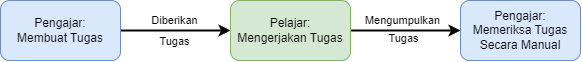
\includegraphics[width=0.8\textwidth]{tradisional.drawio.png}
	\caption[Sistem Tradisional Pemberian Tugas]{Sistem Tradisional Pemberian Tugas}
	\label{fig:1:tradisional}
\end{figure}

Pemberian tugas menulis kode program memiliki banyak masalah. Oleh karena itu, dibutuhkannya sistem baru untuk memberikan tugas kepada pelajar bidang informatika. Sistem baru yang dimaksud tentunya untuk melakukan penilaian secara otomatis. Sebuah sistem yang mengambil kode program pelajar dan memberikan sebuah nilai numerik yang menandakan hasil dari kode program tersebut\footnote{Kurnia, A., Lim, A., dan Cheang, B. (2001) Online judge. {\em Computers \& Education}, {\bf  18}, 299--315.}. Suatu hal yang menarik, Tugas kode program dapat dibagi menjadi 2 jenis yaitu tugas individu dan tugas kelompok. Pada tugas kelompok merupakan tugas yang ditanggung oleh banyak pelajar, biasanya program yang dibuat memiliki antarmuka dan harus diperiksa oleh pengguna khusus yang mengetahui fitur-fitur yang dibutuhkan. Sedangkan tugas individu merupakan sebuah tugas yang diberikan untuk satu individu, biasanya program yang dibuat bersifat algoritmik dan tidak memerlukan antarmuka untuk dijalankan. Program algoritmik sebuah jenis program yang dibuat berdasarkan algoritma untuk menyelesaikan masalah tertentu. Algoritma sendiri adalah langkah-langkah dalam pemecahan masalah secara sistematis\footnote{IDCloudHost (2020) Algoritma pemrograman beserta contohnya.
	\newblock \url{https://idcloudhost.com/blog/algoritma-pemrograman-pengertian-fungsi-cara-kerja-dan-contohnya/}.
	6 Desember 2024.}.
% FIXME: ini kalimat line 16, asa kurang tp buat memperjelas gt 
Algoritma itu seperti resep makanan, dimana akan ada bahan-bahan yang dibutuhkan dan serangkaian langkah untuk membuat suatu makanan yang dijelaskan.

Sebagian besar program yang bersifat algoritmik hanyak perlu mengambil input dari input standar seperti angka, huruf, dan sebuah kata atau kalimat dengan format yang sudah ditentukan, seolah-olah input ini merupakan output dari program lain. Kemudian program algoritmik akan memproses input tersebut dalam komputer dan mengeluarkan hasil komputasinya dalam format yang sudah ditentukan untuk dibaca oleh program lain dan memanfaatkan hasil komputasi tersebut. Singkatnya, program algoritmik itu seperti filter antar program. Dengan ini, sistem penilaian secara otomatis dapat dibuat dengan membuat sebuah program yang mengambil kode program, memasukkan input sesuai format ke dalam program tersebut, membaca hasil keluaran program, dan menilai hasil keluaran program tersebut\footnote{Kurnia, A., Lim, A., dan Cheang, B. (2001) Online judge. {\em Computers \& Education}, {\bf  18}, 299--315.}. Sistem penilaian otomatis \mbox{ini diberikan nama \textit{Online Judge}}. Terlebih lagi sistem ini dapat dilakukan secara \textit{offline} maupun \textit{online}. Gambar \ref{fig:1:onlinejudge} menunjukkan bagaimana \textit{online judge} berintegrasi dengan sistem pemberian tugas yang sudah ada.

\begin{figure}[H]
	\centering
	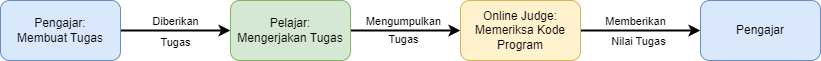
\includegraphics[width=\textwidth]{online_judge.drawio.png}
	\caption[Sistem Integrasi oleh \textit{Online Judge}]{Sistem Integrasi oleh \textit{Online Judge}}
	\label{fig:1:onlinejudge}
\end{figure}

Tugas pemrograman sudah menjadi keseharian dalam pembelajaran pada bidang informatika.
Termasuk pada perguruan tinggi pada bidang informatika, maka \textit{online judge} menjadi sebuah kebutuhan termasuk pada Universitas Katolik Parahyangan atau yang biasa disebut UNPAR.
\textit{Online Judge} yang digunakan oleh UNPAR dinamakan SharIF-Judge\footnote{Vallian, S. (2018) {Kustomisasi Sharif Judge Untuk Kebutuhan Program Studi Teknik Informatika}. Skripsi. Universitas Katolik Parahyangan, Indonesia.} yang merupakan hasil dimodifikasi oleh Stillmen Vallian terhadap Sharif-Judge\footnote{Version 1.4 (2014) {\em Sharif Judge Documentation}. Mohammad Javad Naderi. Tehran, Iran.} buatan Mohammad Javad Naderi yang dibuat menggunakan \textit{framework} CodeIgniter dan Bash. Gambar~\ref{fig:1:dashboardpng} merupakan halaman utama setelah masuk ke dalam SharIF-Judge.

\begin{figure}[H]
	\centering
	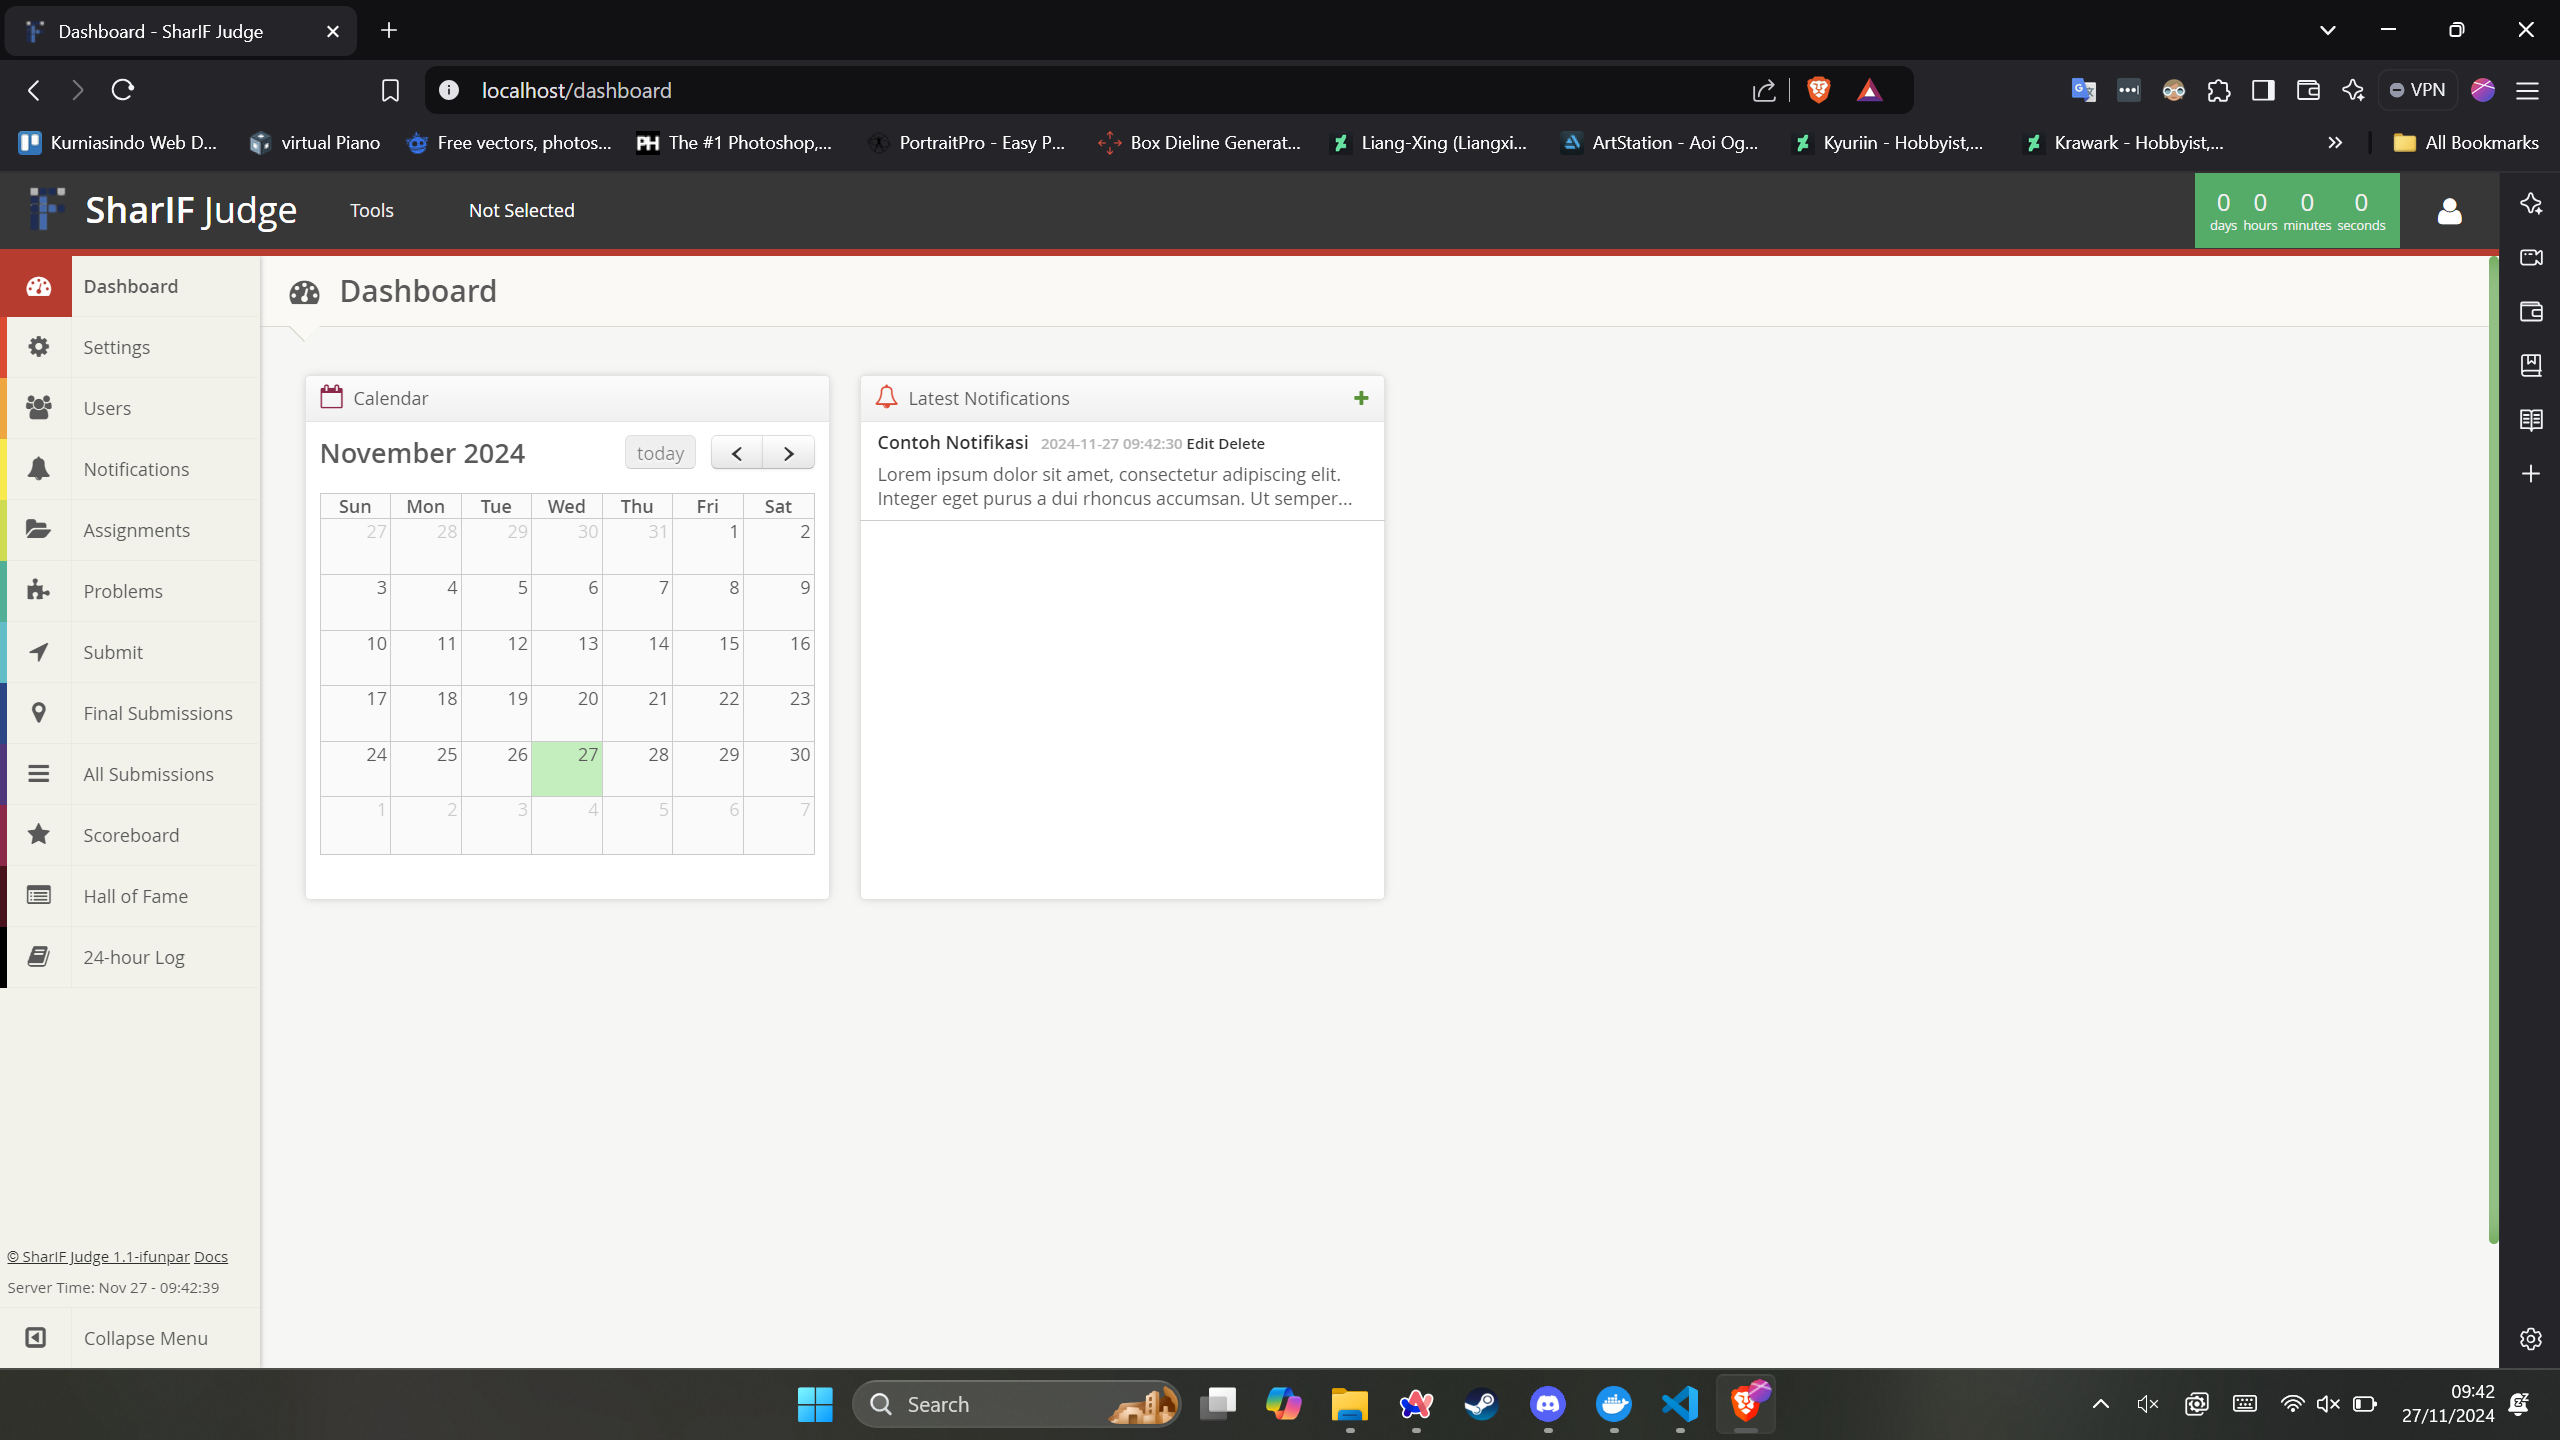
\includegraphics[width=0.8\textwidth]{dashboard.png}
	\caption[Tampilan Awal SharIF Judge]{Tampilan Awal SharIF Judge}
	\label{fig:1:dashboardpng}
\end{figure}

Ujian juga merupakan sebuah bentuk penilaian dari pengajar kepada pelajarnya. Tentunya pelajar maupun mahasiswa ingin memperoleh nilai yang memuaskan dalam ujiannya. Banyak cara yang dilakukan oleh pelajar maupun mahasiswa untuk memperoleh nilai tersebut, salah satunya adalah dengan melakukan kecurangan yaitu \textit{copy paste} atau menyalin jawaban teman atau rekan mereka\footnote{Prihatini, F.~N. dan Indudewi, D. (2016) {Kesadaran dan Perilaku Plagiarisme dikalangan Mahasiswa(Studi pada Mahasiswa Fakultas Ekonomi Jurusan Akuntansi Universitas Semarang)}. {\em Dinamika Sosial Budaya}, {\bf  18}, 68--75.}. Praktek ini diperparah jika ujian dilakukan secara \textit{online}, dikarenakan pelajar dapat mengakses berbagai fasilitas di internet. Oleh karena itu, diperlukanyna sebuah sistem pada sistem \textit{online judge} untuk mengawasi saat terjadinya ujian online.

Pada saat siswa mengerjakan tugas maupun ujian pembuatan kode program, umumnya pengerjaan kode tersebut dilakukan pada aplikasi eksternal seperti \textit{visual studio code} atau \textit{notepad}. Hal ini juga terjadi pada sistem dalam UNPAR dimana mahasiswa akan membuat kode program pada aplikasi eksternal. Ini membuat pengawasan saat pembuatan kode program lebih sulit untuk dilakukan, terlebih jika ujian dilakukan secara \textit{online}. Maka dari itu, Nicholas Aditya Halim memodifikasi SharIF Judge agar semua sistem pemberian tugas seperti pada gambar \ref{fig:1:onlinejudge} dapat dilakukan dalam sistem yang sama yaitu pada SharIF Judge. Sistem yang bangun oleh Nicholas Aditya Halim adalah ``Implementasi editor kode pada Sharif Judge''\footnote{Halim, N.~A. (2021) {Implementasi Editor Kode pada SharIF Judge}. Skripsi. Universitas Katolik Parahyangan,  Indonesia.}, dimana SharIF Judge ditambahkan sebuah \textit{Integrated Development Environment} atau yang disebut dengan IDE. IDE merupakan sebuah sistem yang memiliki kemampuan untuk membuat kode dalam editor kode dan menjalankan kode program tersebut. Dengan adanya IDE, seluruh proses pembuatan kode program dapat dilakukan dalam SharIF Judge. Maka dari itu, seluruh proses sistem pemberian tugas dapat dilakukan dalam satu sistem saja, yaitu SharIF Judge.

Walaupun begitu, pada dasarnya IDE tidak dapat mengawasi jika terjadinya praktek \textit{copy paste}. Maka dari itu pada Tugas akhir ini, IDE pada SharIF Judge akan dimodifikasi untuk menangani hal tersebut dengan ditambahkannya fitur untuk merekam semua ketikan atau kejadian dalam editor kode dalam IDE. Lalu ketikan atau kejadian dalam editor dapat di putar kembali seperti rekaman. Fitur ini akan membuat pengawasan terhadap kegiatan kuliah lebih mudah untuk pengawas dan dapat menjadi bukti kecurangan jika dibutuhkan.

\section{Rumusan Masalah}

Rumusan Masalah yang akan dibahas pada tugas akhir ini adalah:
\begin{enumerate}
	% \item Bagaimana agar editor kode lebih mudah untuk dipakai oleh mahasiswa.
	\item Bagaimana mengimplementasikan perekaman dan pemutaran ulang ketikan mahasiswa pada IDE SharIF-Judge?
	\item Bagaimana cara menyimpan data pemutaran ulang mahasiswa secara rutin dengan otomatis dan tidak mengambil penyimpanan \textit{database} sangat besar?
	\item Bagaimana tanggapan pengguna terhadap implementasi perekaman dan pemutaran ulang kode ketikan pada SharIF Judge?
\end{enumerate}

\section{Tujuan}

Tujuan yang ingin dicapai skripsi ini adalah sebagai berikut:
\begin{enumerate}
	\item Mengimplementasikan perekaman dan pemutaran ulang ketikan mahasiswa pada IDE SharIF-Judge.
	\item Mencari cara penyimpanan data efektif dan mengimplementasikannya pada perekaman dan pemutaran ulang ketikan.
	\item Mendapatkan umpan balik dari tanggapan pengguna terhadap perekaman dan pemutaran ulang ketikan mahasiswa pada SharIF-Judge.
\end{enumerate}

\section{Detail Perkembangan Pengerjaan Skripsi}
Detail bagian pekerjaan tugas akhir sesuai dengan rencan kerja/laporan perkembangan terkahir :
\begin{enumerate}
	\item \textbf{Melakukan studi literatur mengenai bahasa pemrograman PHP.}\\
	      {\bf Status :} Ada sejak rencana kerja skripsi.\\
	      {\bf Hasil :} Bahasa pemrograman PHP sudah dipelajari.

	      PHP atau \textit{Hypertext Preprocessor} merupakan sebuah \textit{scripting language} yang dibuat untuk web development\footnote{https://www.php.net/}. Awalnya PHP dibuat oleh Denmark-Kanada dan Rasmus Lerdorf pada tahun 1993 dan dirilis pada tahun 1995.

	      \textit{File} php akan memiliki extensi \verb|php| seperti contohnya adalah \verb|index.php|. Biasanya \textit{file} PHP akan di proses pada web servernya oleh sebuah PHP \textit{interpreter}. Berikut merupakan contoh kode php. Pada \textit{file} php, tag \verb|<?php| menandakan dimana php \textit{interpreter} akan menterjemahkan teks menjadi kode php, sedangkan diluar

	      \begin{lstlisting}[language={php}, caption={Contoh Sederhana \textit{File} PHP}, label={kode:5:simplephp}]
		  <? php
			echo 'Hello World'
		  ?>
		  \end{lstlisting}

	      %   https://www.freecodecamp.org/news/the-php-handbook/
	      % https://en.wikipedia.org/wiki/PHP#


	\item \textbf{Melakukan studi literatur mengenai \textit{framework} CodeIgniter 3.} \\
	      {\bf Status :} Ada sejak rencana kerja skripsi.\\
	      {\bf Hasil :}

	\item \textbf{Melakukan studi literatur mengenai editor kode Ace.} \\
	      {\bf Status :} Ada sejak rencana kerja skripsi.\\
	      {\bf Hasil :}

	\item \textbf{Melakukan studi literatur mengenai cara penyimpanan rekaman ketikan.} \\
	      {\bf Status :} Ada sejak rencana kerja skripsi.\\
	      {\bf Hasil :}

	\item \textbf{Melakukan studi literatur mengenai SharIF Judge.}\\
	      {\bf Status :} baru ditambahkan pada semester ini\\
	      {\bf Hasil :}

	\item \textbf{Memodelkan dan merencanakan perubahan pada structur website dan database pada SharIF-Judge.} \\
	      {\bf Status :} Ada sejak rencana kerja skripsi.\\
	      {\bf Hasil :}

	\item \textbf{Menulis dokumen skripsi}\\
	      {\bf Status :} Ada sejak rencana kerja skripsi.\\
	      {\bf Hasil :}


\end{enumerate}

\section{Pencapaian Rencana Kerja}
Langkah-langkah kerja yang berhasil diselesaikan dalam Skripsi 1 ini adalah sebagai berikut:
\begin{enumerate}
	\item
	\item
	\item
\end{enumerate}



\section{Kendala yang Dihadapi}
%TULISKAN BAGIAN INI JIKA DOKUMEN ANDA TIPE A ATAU C
Kendala - kendala yang dihadapi selama mengerjakan skripsi :
\begin{itemize}
	\item Terlalu banyak melakukan prokratinasi
	\item Terlalu banyak godaan berupa hiburan (game, film, dll)
	\item Skripsi diambil bersamaan dengan kuliah ASD karena selama 5 semester pertama kuliah tersebut sangat dihindari dan tidak diambil, dan selama 4 semester terakhir kuliah tersebut selalu mendapat nilai E
	\item Mengalami kesulitan pada saat sudah mulai membuat program komputer karena selama ini selalu dibantu teman
\end{itemize}

\vspace{1cm}
\centering Bandung, \tanggal\\
\vspace{2cm} \nama \\
\vspace{1cm}

Menyetujui, \\
\ifdefstring{\jumpemb}{2}{
	\vspace{1.5cm}
	\begin{centering} Menyetujui,\\ \end{centering} \vspace{0.75cm}
	\begin{minipage}[b]{0.45\linewidth}
		% \centering Bandung, \makebox[0.5cm]{\hrulefill}/\makebox[0.5cm]{\hrulefill}/2013 \\
		\vspace{2cm} Nama: \pembA \\ Pembimbing Utama
	\end{minipage} \hspace{0.5cm}
	\begin{minipage}[b]{0.45\linewidth}
		% \centering Bandung, \makebox[0.5cm]{\hrulefill}/\makebox[0.5cm]{\hrulefill}/2013\\
		\vspace{2cm} Nama: \pembB \\ Pembimbing Pendamping
	\end{minipage}
	\vspace{0.5cm}
}{
	% \centering Bandung, \makebox[0.5cm]{\hrulefill}/\makebox[0.5cm]{\hrulefill}/2013\\
	\vspace{2cm} Nama: \pembA \\ Pembimbing Tunggal
}
\end{document}

